\subsection{Интеграция ИИ-модуля DeepSeek в архитектуру проекта}

Для обеспечения эффективной работы ИИ-компонента в образовательной платформе реализована модульная архитектура с чётким разделением ответственности. Последующие подразделы детализируют ключевые аспекты интеграции: стратегию контейнеризации для изоляции сервиса, механизмы взаимодействия с клиентской частью и системные преимущества выбранного подхода. Основное внимание уделено сохранению прозрачности работы ИИ для конечных пользователей при обеспечении гибкости разработки и эксплуатации.

\subsubsection{Контейнеризация DeepSeek}
Для обеспечения независимого жизненного цикла и лёгкой масштабируемости ИИ-компонента DeepSeek развёртывается в виде изолированного Docker-контейнера. Такой подход позволяет:

\begin{itemize}
  \item быстро запускать и останавливать сервис без влияния на основное приложение;
  \item поддерживать разные версии DeepSeek параллельно, экспериментируя с обновлениями моделей;
  \item мигрировать между хостами и облачными средами с минимальными изменениями конфигурации.
\end{itemize}

\subsubsection{Преимущества контейнеризированного подхода}
Контейнеризация DeepSeek даёт следующие ключевые плюсы:
\begin{itemize}
  \item Изоляция нагрузки: анализ кода выполняется в отдельном окружении, не влияя на отзывчивость интерфейса;
  \item Горизонтальное масштабирование: при большом числе запросов можно запускать несколько инстансов контейнера;
  \item Упрощённое сопровождение: обновление ИИ-компонента сводится к выпуску нового Docker-образа без правок во фронтенде;
  \item Гибкость развертывания: контейнеры можно запускать локально и в облаке с одинаковой конфигурацией.
\end{itemize}

\subsubsection{Взаимодействие клиентской части с DeepSeek}

Клиентская часть приложения, реализованная на React и Next.js, отправляет HTTP-запросы к back-end части Web-приложения при прикреплении решения задания студентом, далее back-end автоматически начинает проверку решения при помощи анализ на основе искусственного интеллекта. Результат проверки приходит пользователю при запросе на получения детальной информации по задаче, выполненной студентом.

\begin{figure}[h]
    \centering
    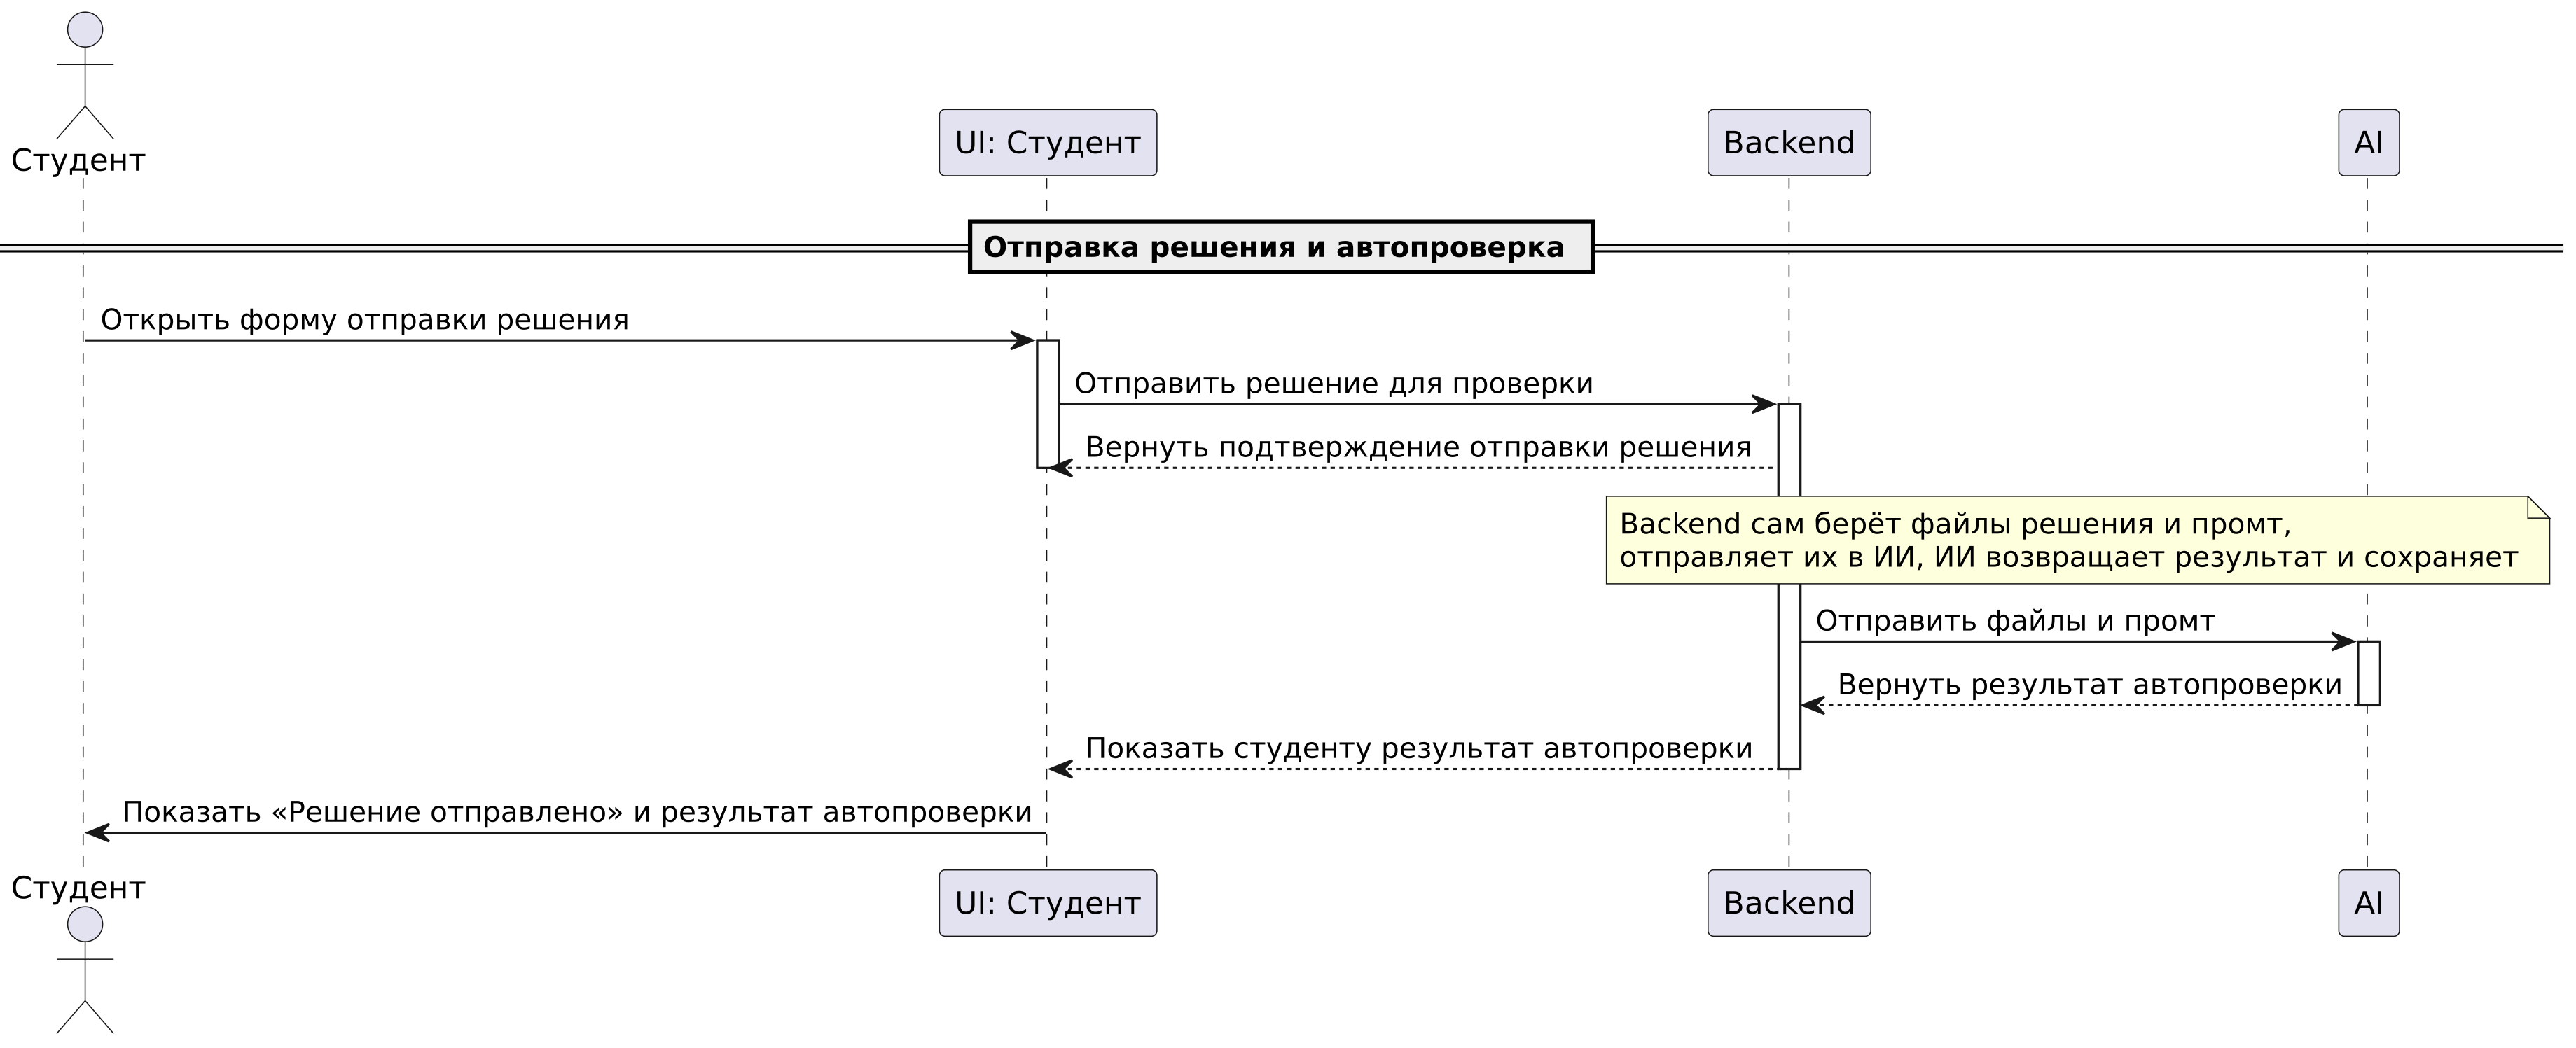
\includegraphics[width=0.8\linewidth]{static/diagrams/TaskSendStudentDiagram.png}
    \caption{Схема взаимодействия клиентской части (React/Next.js) с модулем DeepSeek}
    \label{fig:client-deepseek}
\end{figure}

На рисунке \ref{fig:client-deepseek} представлена схема взаимодействия клиентской части с модулем DeepSeek.

\subsubsection{Вывод}

Контейнеризация DeepSeek обеспечивает полную независимость остальных компонентов приложения от ИИ-модуля, позволяя развёртывать и обновлять его без влияния на другие сервисы. Взаимодействие через API бэкенда создаёт своего рода «чёрный ящик» для клиента, что упрощает инкапсуляцию логики и даёт гибкость в распределении и масштабировании нагрузки на контейнер с ИИ.


